\documentclass{aamas2010_cameraReady}

%\usepackage{times}
\usepackage{latexsym}
\usepackage{amsfonts,amsmath,amssymb}
\usepackage{graphicx}
\usepackage{algorithmic}
\usepackage{subfigure}



\newtheorem{Theorem}{Theorem}
\newtheorem{Lemma}{Lemma}
\newtheorem{Example}{Example}
\newtheorem{Corollary}{Corollary}
\newtheorem{Definition}{Definition}
\newtheorem{assume}{Assumption}
\newtheorem{Proposition}{Proposition}
\newtheorem{Hypothesis}{Hypothesis}


\special{papersize=8.5in,11in}

\pdfpagewidth=8.5truein
\pdfpageheight=11truein

\begin{document}

\AuthorsForCitationInfo{Z. Rabinovich, L. Dufton, K. Larson and N. R. Jennings}

\TitleForCitationInfo{Cultivating Desired Behaviour}%: Policy Teaching Via Environment-Dynamics Tweaks}


\title{Cultivating Desired Behaviour:\\ Policy Teaching Via Environment-Dynamics
 Tweaks}


% AUTHORS
\def\sharedaffiliation{%
\end{tabular}
\begin{tabular}{c}}
%
\numberofauthors{4}
\author{\alignauthor Zinovi Rabinovich$^{\dagger}$\\
  \email{zr@ecs.soton.ac.uk}
\alignauthor Lachlan Dufton$^*$\\ 
  \email{ltdufton@cs.uwaterloo.ca}
\alignauthor Kate Larson$^*$\\
  \email{klarson@cs.uwaterloo.ca}
\and
\alignauthor Nicholas R. Jennings$^{\dagger}$\\
  \email{nrj@ecs.soton.ac.uk}
\sharedaffiliation
  \affaddr{$^{\dagger}$Electronics and Computer Science, University of Southampton, United Kingdom}\\
  \affaddr{$^*$Cheriton School of Computer Science, University of Waterloo, Canada}\\
} 
%\additionalauthors{}
%\author{Tracking Number: 398}


\maketitle

\begin{abstract}

In this paper we study, for the first time explicitly, the
implications of endowing an interested party (i.e. a teacher) with the
ability to modify the underlying \emph{dynamics} of the environment,
in order to encourage an agent to learn to follow a specific
policy. We introduce a cost function which can be used by the teacher
to balance the modifications it makes to the underlying environment
dynamics, with the learner's performance compared to some ideal,
desired, policy. We formulate teacher's problem of determining optimal
environment changes as a planning and control problem, and empirically
validate the effectiveness of our model.

\end{abstract}

\category{I.2.6}{Artificial Intelligence}{Learning}
\category{I.2.8}{Artificial Intelligence}{Problem Solving, Control Methods, and 
Search}[Control theory]
\category{I.2.11}{Artificial Intelligence}{Distributed Artificial Intelligence}[
Multiagent systems]
\terms{Algorithms}
\keywords{Teacher-learner, control theory, Kullback-Leibler Rate}



\section{Introduction}
%\nocite{fleming_hernandez-hernandez_CDC_97}
%\nocite{todorov_2009_framework_sup}
%\nocite{todorov_2009_framework}
%\nocite{ng_russell_2000}
%\nocite{zhang_parkes_2009_ed}
%\nocite{dufton_larson_2009}

There are three main teaching techniques applied by people: by
demonstration, by incentive, by environment dynamics
modification. While the
first two have been mapped into intelligent agent models, to the best
of our knowledge, the third one has yet to be instantiated.

Teaching by {\em demonstration} has found a significant expression in
robotics~\cite{argal_etal_2009}. However, most of these works assume
that the learner actually wishes to learn the task, as well as a
certain benevolence on behalf of the teacher with respect to the
learned task.

On the other hand, teaching by {\em incentive} has been formalised in a way
that allows to the teacher to have an interest that may contradict
that of the learner. In more detail, recently, Zhang \emph{et al}
introduced a general framework for \emph{environment
  design}~\cite{Zhang09:General}. In environment design an interested
party attempts to influence the behaviour of an agent by making limited
changes to the agent's environment. Although in general this may
include environment dynamics modification, Zhang \emph{et al} have
concentrated on teaching by incentive. In particular, Zhang \emph{et
  al} have allowed their interested party to modify the cost function
of an agent in a linear programming example~\cite{Zhang09:General}, or
to modify the rewards of an agent acting in an environment modelled as
a Markovian Decition Problem (MDP)~\cite{zhang_parkes_2008,Zhang09:Policy}.

In this paper we explicitly focus on the the implications of allowing
the interested party (teacher, in our model) to modify the
\emph{dynamics} of the environment, while leaving the reward function
of the agent alone. We term this process of teaching {\em behaviour
  cultivation}. In more detail, we concentrate on environments
modelled by the learner as an MDP, and allow the teacher to tweak the
environment dynamics and record the outcome within the MDP model. The
teacher's goal is, therefore, to determine the form and the degree of
tweaking necessary to enforce a specified behaviour upon the
learner. To achieve this goal, we first introduce a way to measure the
divergence between the realised and the passive (when no modification
is applied by the teacher) environment developments in a Markovian
system. This measure naturally incorporates and balances the teacher's
effort and the deviation of the learner's performance from an ideal
reference, that which the teacher is interested in. It also allows us
to formulate the teacher's problem as a planning and control problem,
and solve it using classical analytical and numerical tools.

While our model may be cast as an example of environment design, we
note that our instantiation differs significantly from the particular
cases studied by Zhang \emph{et al}, and therefore creates a separate
line of study. In fact, representing the teacher's task as a control
problem is far more reminiscent of the work by Banerjee and
Peng~\cite{banerjee_peng_2005}, although it too focuses on the reward
modification.

To realise the necessity and importance of teaching by environment
dynamics modification consider the following real life scenario. A
parent wishes to teach a child to ride a bicycle. The parent may {\em
  demonstrate} by riding the bicycle. However, in practice, this does
not yield good results when the child attempt to repeat the task. It
is also possible to promise an {\em incentive}, be that a candy or a
trip to the movies. Unfortunately, although increasing the child's
efforts, this does not facilitate the learning process. The most
practical thing to do in this case, is to {\em modify the dynamics} --
add safety wheels to the bicycle. Gradually raising the safety wheels
constitues {\em behaviour cultivation}. It ultimately allows the child
to accustom to the complete range of motion possibilities and,
eventually, ride an unabridged bicycle version.

In what follows we will formally define {\em behaviour cultivation}
process that can be parameterised by the learning algorithm we wish to
teach(Section~\ref{sec: GeneralModel}).
%teaching by dynamics
%modification 
%given a learning algorithm we wish to teach
%. 
We will also provide a specialised
version of the formalism for a specific MDP solution technique --
Policy Iteration (PI) algorithm (Section~\ref{sec: TOP-PI}). $\{\{$
Our experiments in Section~\ref{sec: experiments} will compare the
performance of PI with and without dynamics modification. $\}\}$. We
will then conclude in Section~\ref{sec: future work} with a discussion
of further development teaching by dynamics modification.




%%%%%%%%%%%%%%%%%%%%%%%%%%%%%%
\section{Interaction Model}\label{sec: GeneralModel}
%%%%%%%%%%%%%%%%%%%%%%%%%%%%%%

In this section we provide a high level description of the problem and
general framework.  In the next section we provide a particular
instantiation of our framework.

For easier exposition we will present our framework to consist of a
stochastic environment and two agents, a \emph{learner} and a
\emph{teacher}, however, our formalism can be easily modified to
include an arbitrary fixed number of learning agents. The learner acts
within the environment, taking actions and receiving feedback in the
form of rewards, which depend on the action taken and the current
state of the environment in which the agent finds itself.  We assume
that the learner is rational and thus attempts to find a \emph{policy}
which describes what action to take in each environment state, so as
to maximise its expected reward.  The teacher, on the other hand,
does not act \emph{in} the environment, but rather acts \emph{on} the
environment.  In particular, the teacher has some desired
\emph{reference policy}, $\pi^*$, that it wishes the learner to
follow, but is unable to directly force the agent to take any
particular action.  Instead, it it is able to modify the environment's
\emph{dynamics} in order to cultivate the desired behaviour in the
learner.  That is, the teacher's actions are able to influence the way
the environment state changes in response to the learner's actions,
and thus influence the policy of the learner. This influence can range
from minor effects on the transition probability in a single
environment state to a principal change of the environment response
across all states and learner's actions. Dynamics modifications, or
\emph{tweaks}, come at a cost, however, and thus the goal of the
teacher is to minimise the modifications it must make to the
environment dynamics while at the same time ensuring that the policy
followed by the learner is close enough to the desired reference
policy.

We represent  the problem with the tuple  $\langle S, A, c,\gamma, U,T\rangle$ where:
\begin{itemize}
\item $S$ is the set of states, 
\item $A$ is the set of actions available to the learner,
\item  $c:S\times A\times S\rightarrow\mathbf{R}$ is the reward (or
  cost) function of the learner. $c(s',a,s)$ is the reward received by
  the learner if it has applied action $a\in A$ and the environment
  moved from state $s\in S$ to state $s'\in S$,
\item $\gamma \in (0,1)$ is a discount factor,   

\item $U$ is the set of actions (modifications to the environment)
  that the teacher can apply where $u_t\in U$ is the modification or tweak made
  at time $t$,

\item $T:S\times A\times U\rightarrow\Delta(S)$ describes the
  environment dynamics where $T_u(s'|s,a)\equiv T(s'|s,a,u)$ is the
  probability that the state will change from $s$ to $s'$ if the
  learner has applied action $a\in A$ and the teacher chose
  environment modification $u\in U$.

We assume that there exists a null modification $u^0\in U$, so that
$T^0=T_{u^0}$ are the original dynamics of the environment before any
teacher-modifications. We will use the term \emph{passive dynamics} to
refer to $T^0$ to highlight the fact that it is unchanged by the teacher.

\end{itemize}

We assume that the learner modifies and updates its policy by using
some iterative algorithm, such as value or policy iteration.  In
between iterations, the teacher is able to apply a tweak or
modification to the environment dynamics, and thus, the learner faces
a sequence of Markov Decision Problems (MDPs)~\cite{puterman_book_94},
given by tuples $<S,A,U,T_{u_t},R>$. We assume that the learner is
unaware of the teacher's actions, and thus proceeds as if the sequence
of MDPs were homogeneous.
 
 
\begin{assume}\label{assume_persistence}
At every stage the learner seeks an action policy of the form
$\pi:S\rightarrow\Delta(A)$ that would produce the highest expected
reward if $T_{u_t}$ would persist indefinitely.\footnote{This
  assumption is explicit only if the learner actually has access to
  the environment model. For most standard reinforcement learning
  algorithms this assumption would hold implicitly.}
\end{assume}


Let $x_t$ represent all information and features that the learner uses
in determining its policy, and let
$\pi_t=\pi(x_t):S\rightarrow\Delta(A)$ be the policy that corresponds
to that state.  Additionally, let $\pi^*$ be the ideal policy that the
teacher desires the learner to follow.  At time $t$, the teacher
incurs a cost, $\mathrm{Cost}(\pi_t,u_t)$, which combines the
difference between the actual policy being followed by the learner,
$\pi_t$, and the policy desired by the teacher, $\pi^*$, with the
amount of environmental modifications the teacher has had to make in
order to maintain the current dynamics, $T_{u_t}$, compared to the
initial environment dynamics, $T^0$. If we let $x_t=F(x_{t-1},u_t)$
denote one step of the learner's policy-determination algorithm and
assume that $x_0$, the original state of the learner, is known, then
it is possible to formulate the overall optimisation problem faced by
the teacher.  In particular, it is:
\begin{eqnarray*}
&\min\limits_{u_t}\sum\limits_{t=1}^{t_{max}}Cost(\pi_t,u_t)\\
&s.t.\\
&\pi_t=\pi(x_t)\\
&x_t=F(x_{t-1},u_t).
\end{eqnarray*}



%Now, denote $x_t$ the internal state of the learner's policy
%computation at iteration $t$, and let
%$\pi_t=\pi(x_t):S\rightarrow\Delta(A)$ be the policy that corresponds
%to that computation state. Also, denote $\pi^*$ the ideal reference
%action policy of the learner. Then at time $t$ the teacher incurs cost
%$Cost(\pi_t,u_t)$ that combines the distance between $\pi_t$ and
%$\pi^*$ and between $T_{u_t}$ and $T^0$. The overall optimisation
%problem for the teacher is as follows, where $x_t=F(x_{t-1},u_t)$
%denotes one step of the learner's computation algorithm and $x_0$ is
%known:
%\begin{eqnarray*}
%&\min\limits_{u_t}\sum\limits_{t=1}^{t_{max}}Cost(\pi_t,u_t)\\
%&s.t.\\
%&\pi_t=\pi(x_t)\\
%&x_t=F(x_{t-1},u_t)
%\end{eqnarray*}

This formulation of the teacher's optimisation function is fully
generic. It does not explicitly specify the learner's algorithm beyond
assuming that it is iterative. This formalism thus captures both
policy and value iteration algorithms, both with given and learned
environment models.  It can also capture the case where the learner is
capable of transfer learning~\cite{ taylor_stone_2009}. In this
scenario the learner's state $x_t$ will include structural knowledge
gathered thus far from the interaction with the environment.

Our teacher-learner interaction framework, as described, is also
generic with respect to the instantiation of the teacher's cost
function, $Cost(\pi_t,u_t)$. We argue that suitable cost functions for
this problem should incorporate information as to what environmental
modifications the teacher has performed (\emph{i.e.} the actions taken
by the teacher), along with information about how similar the policy
of the learner is to the desired policy of the teacher (\emph{i.e.}
how far the teacher is from its goal). While any function which
combines these features in a meaningful way would work, in this paper
we adopt a specific cost function derived from the
\emph{Kullback-Leibler Divergence Rate}.  We describe our proposed
cost function and the reason behind our cost function choice in more
detail in the next section.



\subsection{Teacher's Cost Computation}\label{sec:KLCost}

In this section we describe our cost function, based on the
Kullback-Leibler Divergence Rate (KL Rate or KLR).  We first provide some
background material on Kullback-Leibler Divergence (KL Divergence) and
KLR. We then describe how our cost function is defined, and provide an
argument as to why it is appropriate for our setting.


\begin{Definition}
Let $p$ and $q$ be probability distributions over some discrete random
variable. Then the Kullback-Leibler (KL) Divergence of $q$ from $p$ is
\[
D^{KL}(p||q)=\sum_i p(i)\log \frac{p(i)}{q(i)}.
\]
\end{Definition}

\noindent Informally, KL Divergence measures the difference between
two probability distributions.  KL Rate is an extension of KL
Divergence to Markov processes.
\begin{Definition}
Let $\{X^1_t\}$ and $\{X^2_t\}$ be Markov Processes.  The
Kullback-Leibler (KL) Rate is
\[
KLR(X^1||X^2)=\lim_{n\rightarrow \infty} \frac{1}{n}DL^{KL}(P(X^1=x_n)||P(X^2=x_n)).
\]
\end{Definition}
If the processes can be described by two conditional transition
matrices, $P$ and $Q$, where $P(x'|x)$ (and respectively $Q(x'|x)$) is
the probability of transitioning from state $x$ to state $x'$, then
\[
KLR(X^1||X^2)=\sum_{x} D^{KL}(P(\cdot|x)||Q(\cdot|x))p_{stat}(x)
\]
where $p_{stat}$ is the stationary distribution of
$P$~\cite{rached_alajaji_campbell_2004}.


Now, returning to our problem, let $\pi_t$ be the policy of the
learner at time $t$ and let $T_{u_t}$ be the dynamics of the
environment after the teacher has applied tweak $u_t$. If $\pi_t$ was
to be repeatedly used in the environment modified by $u_t$, this would
result in a homogeneous Markovian process defined by the transition
matrix
\[
P_t(s',a'|s,a)=T_{u_t}(s'|s,a)\pi_t(a'|s').
\]
Similarly, we can define another  Markovian process by the transition matrix
\[
P^*(s',a'|s,a)=T^0(s'|s,a)\pi^*(a'|s').
\]
This is the ideal stochastic process over state-action pairs, from the
teacher's perspective. In particular, it is formed when the teacher's
desired policy, $\pi^*$, is followed by the learner in the original,
unmodified environment. That is, the learner executes the teacher's
desired policy with no intervention from the teacher.

Assuming that $P_t$ and $P^*$ are irreducible with respect to $S\times
A$, we define our cost function as
\begin{eqnarray*}
Cost(u_t,\pi_t) & =& KLR(P_t||P^*) \\
                           &=& \sum_{s,a}D^{KL}_t(s,a)q_t(s,a)
\end{eqnarray*}
where
\[
D_t^{KL}(s,a)=D^{KL}(P_t(\cdot,\cdot|s,a)||P^*(\cdot,\cdot|s,a))
\]
and $q_t(s,a)$ is the  stationary distribution of $P_t$, so that
$q_t=P_tq_t$. 
Notably, the
stationary distribution can be decomposed (with a slight abuse of
notation) to be $q_t(s,a)=q_t(a|s)q_t(s)$ and then expressed by the
following equations:
%% \begin{eqnarray*}
%% q_t&=&q_t(a'|s')q_t(s')=P_tq_t\\
%% &=&\sum\limits_{s,a}T_{u_t}(s'|s,a)\pi_t(a'|s')q_t(a|s)q_t(s)\\
%% &=&\pi_t(a'|s')\sum\limits_sq_t(s)\sum\limits_aT_{u_t}(s'|s,a)q_t(a|s)\\
%% &&\{\displaystyle{substitute}\ \ q_t(\cdot|\cdot)\Leftarrow\pi_t(\cdot|\cdot)\}\\
%% &=&\pi_t(a'|s')\sum\limits_sq_t(s)\sum\limits_aT_{u_t}(s'|s,a)\pi_t(a|s)\\
%% &&\{\displaystyle{denote}\ \ \Tilde{T}_{u_t}(s'|s)=\sum\limits_aT_{u_t}(s'|s,a)\pi_t(a|s)\}\\
%% &=&\pi_t(a'|s')\sum\limits_sq_t(s)\Tilde{T}_{u_t}(s'|s)
%% \end{eqnarray*}
%% so that
\begin{eqnarray*}
q_t(s',a')&=&\pi_t(a'|s')q_t(s')\ \ \mbox{where}\\
q_t(s')&=&\sum\limits_s\Tilde{T}_{u_t}(s'|s)q_t(s) \ \ \mbox{and}\\
\Tilde{T}_{u_t}(s'|s)&=&\sum_{a}T_{u_t}(s'|s,a)\pi_t(a|s).
\end{eqnarray*}



Incorporating our KLR-based cost function, the overall generic Teacher
Optimisation Problem (TOP) is depicted in Figure~\ref{t_opt}. 

Notice that this formulation retains complete flexibility with respect
to the specific algorithm selected by the learner to optimise its
policy. Nevertheless, to provide further intuition and demonstrate the
feasibility of the approach, in the rest of this paper we instantiate
the algorithm $F$ to be the Policy Iteration (PI) algorithm. As would
occur with any other learning algorithm, we will identify $x_t$ with a
set of variables sufficient to capture the learner's computation state
at iteration $t$. We then will represent the change in the computation
state that occurs between two sequential iterations of the algorithm in
a functional form, $F$. The choice of PI is, therefore, not dictated
by its particularly convenient properties, but rather by the number of
applications it has been used in. As we discuss in the next section,
by using PI as our example instantiation of TOP we intend to speed up the 
dissemination and utilisation of our {\em behaviour cultivation}
teaching method to practical applications. However, before proceeding
to this particular instantiation of TOP to PI, we would like to remark
upon the meaning of the use of KLR and KL Divergence in our teaching
problem.

%%%%%%%%%%%%%%%%%
\begin{figure}[ht]
\begin{tabular}{|c|} \hline \parbox{3.2 in} {\center 
$\arg\min\limits_{u_t}\sum\limits_{t=1}^{t_{max}}\sum\limits_{s,a}\pi_t(a|s)q_t(s)D^{KL}_t(s,a)$\\
s.t.\\
$\pi_t=\pi(x_t)$\\
$x_t=F(x_{t-1},u_t)$\\
$x_0\ \ \displaystyle{is\ \ given}$\\
$D^{KL}_t(s,a)=\sum\limits_{s',a'}T_{u_t}(s'|a,s)\pi_t(a'|s')\log\frac{T_{u_t}(s'|a,s)\pi_t(a'|s')}{T^0(s'|a,s)\pi^*(a'|s')}$\\
$q_t(s')=\sum\limits_s\Tilde{T}_{u_t}(s'|s)q_t(s)$\\
$\Tilde{T}_{u_t}(s'|s)=\sum\limits_aT_{u_t}(s'|s,a)\pi_t(a|s)$\\\ \\
}\\ \hline \end{tabular}
\caption{\label{t_opt}The complete generic TOP}
\end{figure}
%%%%%%%%%%%%%%%%%%%%%%%%%%%%%%

As we have mentioned in the start of this section, KL Divergence,
$D^{KL}(P||Q)$, informally measures the difference between some
factual distribution $P$ and some desired distribution
$Q$.\footnote{Note that while KL Divergence is often called the
  \emph{distance} between two distributions, it is, in fact, not a
  true distance metric.}  As expected, $D^{KL}(P||Q)$ is minimised
exactly when $P=Q$, that is, $D^{KL}(P||P)=0$. Importantly, it
compares two distributions, rather than distribution properties, such
as the mean or variance which, for historical reasons, have been more commonly
used.\footnote{Consider, for instance, the optimality criteria of
  MDPs: the {\em expected} accumulated reward. Rather than being
  concerned with the entire shape of the obtainable reward
  distribution, it only concentrates on the expectation, necessitating
  further solution augmentation to account for requirements such as
  risk-aversion.}  In our problem, the desired distribution is
$P^*(s',a'|s,a)$ which arises if the learner follows the teacher's
desired policy with no environmental tweaks required.  By using KLR as
the cost function, we are able to assign costs to the complete variety
of possible long term deviations caused by departing from the ideal
probability of state-action pair transition.  These deviations may
arise from either the environmental tweak made by the teacher, or by
the learner following a non-desired policy, or some combination of
both, and thus our cost function balances these appropriately.

%Originally, $KL$ divergence (and KRL) was designed to measure the cost
%of mistaken encoding. That is, if a signal had come from a
%distribution $P$, while we have used a distribution $Q$ to encode it,
%$KL(P\|Q)$ measures the extra bits we had to
%use\cite{cover_thomas_IT_book_91}. Therefore, given the signal,
%information theory seeks to recover $Q$ to minimise the extra cost. In
%our teaching domain, the signal is the sequence of state-action pairs
%engendered by the system dynamics and the learning algorithm. However,
%by changing the system dynamics we essentially change the signal true
%distribution, rather than its encoding. Hence, we represent the ideal
%policy and the passive dynamics as the encoding distribution $Q$,
%while we modulate the signal distribution $P$ to match it.






\section{TOP with Policy Iteration}\label{sec: TOP-PI}
The standard policy iteration (PI) algorithm is an iterative algorithm
that operates over an explicitly given MDP\cite{puterman_book_94}, and
it has two principal stages: policy evaluation and policy
improvement. At the the {\em policy evaluation} stage PI computes the
reward gained by applying currently considered policy. Specifically,
given the policy of the previous iteration, $\pi_{t-1}$, the value
function $V_t(s)$ for that policy is computed, where $V_t(s)$
represents the expected total discounted reward that can be achieved
if the environment starts at state $s$ and the agent follows
$\pi_{t-1}$. At the {\em policy improvement} stage the value function
of the current policy is used to guide the computation of the next
stage policy. Commonly, it is a policy, $\pi_{t}$, optimal with
respect to the currect value function, $V_t(s)$.

Since its original introduction, both stages of the algorithm have
been refined to enable partial knowledge of the domain or introduce
conservative safety features. For instance, the value function can be
estimated, rather than computed, in environment where a direct
computation is too complex or impossible due to poor modelling by the
learner. Another possible extension is introduction of safety features
into the calculations of the new policy (e.g risk aversion). Such
modifications have been extensively used, particularly in robotics,
leading to more and more advanced methods (see
e.g.~\cite{sugiyama_et_al_2009}). Hence, by making basic PI method our
study subject in this paper, we intend to impact a large cross-cut of
applications where these learning techniques are used in a
teacher-learner (or leader-follower) setup.

In more detail, we consider the standard PI algorithm, where the
environment model is completely known and the value function is
directly computed. However, for the reasons of computational
convenience, we do introduce a modification into the policy
improvement stage. Namely, the new policy is computed as a
soft-maximisation with respect to the value function. The soft-max
function we use is that of Gibbs-Boltzmann, where a vector
$\mathbf{v}=(v_1,...,v_k)$ is tranformed into a normalised vector
$\sigma(\mathbf{v}|\tau)$ proportional to $(\exp(\tau
v_1),...,\exp(\tau v_k))$. The parameter $\tau_t$ denotes a so called
{\em temperature} scale that shifts the soft-max towards the greedy
maximum selection, i.e. if we let
$\lim\limits_{\tau\rightarrow\infty}\sigma(\mathbf{v}|\tau)=\sigma^*$,
then $\sigma^*_j\neq 0$ iff $j\in\arg\max\limits_{1\leq i\leq k}v_i$.

This is done to support differentiability of the policy with respect
to the environment dynamics. Although it may appear as a significant
modification to the standard PI algorithm, it is in fact a quite
common practice. This is due to the fact that PI is frequently used in
combination with a form of neural-network computation to represent
either the policy or the value function, and in such representations
soft-max occurs naturally.

Formally instantiating our learner's state update $F(x_t,u)$ by PI
leads to the following set of equations:\\\ \\
{\em Policy evaluation:}\\
\centerline{
  $V_t(s)=\sum\limits_{s'}T_{u_t}(s'|s,\pi_{t-1}(s))\left[
    c(s',\pi_{t-1}(s),s)+\gamma V_t(s')
    \right]$}
{\em Policy improvement:}\\
\centerline{
$\pi_t(a|s)=\frac{1}{Z_t(s)}\exp\left(\tau_t\sum\limits_{s'}T_{u_t}(s'|s,a)\left[
    c(s',a,s)+\gamma V_t(s')
    \right]\right)$}
{\em Normalisation factor:}\\ 
\centerline{
$Z_t(s)=\sum\limits_a\exp\left(\tau_t\sum\limits_{s'}T_{u_t}(s'|s,a)\left[
    c(s',a,s)+\gamma V_t(s') \right]\right)$}

Substituting the above into the standard
TOP formulation leads to a TOP-PI optimisation problem depicted in
Figure~\ref{t_opt_PI}.
\begin{figure}[th]
\begin{tabular}{|c|} \hline \parbox{3.2 in} {\center 
$\arg\min\limits_{u_t}\sum\limits_{t=1}^{t_{max}}\sum\limits_{s,a}\pi_t(a|s)q_t(s)D^{KL}_t(s,a)$\\
$s.t.$\\
$V_t(s)=\sum\limits_{s'}T_{u_t}(s'|s,\pi_{t-1}(s))\left[
c(s',\pi_{t-1}(s),s)+\gamma V_t(s')
\right]$\\
$\pi_t(a|s)=\frac{\exp\left(\tau_t\sum\limits_{s'}T_{u_t}(s'|s,a)\left[
c(s',a,s)+\gamma V_t(s')
\right]\right)}{Z_t(s)}$\\
$Z_t(s)=\sum\limits_a\exp\left(\tau_t\sum\limits_{s'}T_{u_t}(s'|s,a)\left[
c(s',a,s)+\gamma V_t(s')
\right]\right)$\\
$\pi_0\ \ \displaystyle{given}$\\
$D^{KL}_t(s,a)=\sum\limits_{s',a'}T_{u_t}(s'|a,s)\pi_t(a'|s')\log\frac{T_{u_t}(s'|a,s)\pi_t(a'|s')}{T^0(s'|a,s)\pi^*(a'|s')}$\\
$q_t(s')=\sum\limits_s\Tilde{T}_{u_t}(s'|s)q_t(s)$\\
$\Tilde{T}_{u_t}(s'|s)=\sum\limits_aT_{u_t}(s'|s,a)\pi_t(a|s)$\\\ \\
}\\ \hline \end{tabular}
\caption{\label{t_opt_PI}TOP-PI: The complete and explicit TOP for the
  PI learner}
\end{figure}

\section{Experimental Demonstration}\label{sec: experiments}
Consider a learner agent that is tasked with finding an optimal path
for supply transportation between point $S$ and $T$ on a grid. The
learner's reward is initially fixed to be $-1$ for every step it takes
plus some values $R_{ST}$ and $R_{TS}$ for reaching point T from S and
vice versa. In a uniform grid this would be a simple problem, however,
the grid simulates a terrain and cells have an associated elevation.  
As a result, any movement from one cell to another neighbouring cell
succeeds with a probability proportional to the relative elevation of 
the cells. Consider the situation depicted in Figure~\ref{exp_motion}. 

\begin{figure}[ht]
\centerline{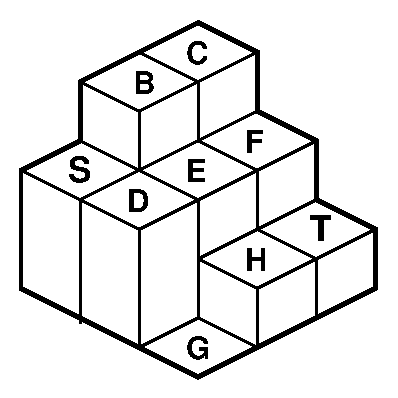
\psfig{file=img/exp_motion.eps,width=5cm}}
\caption{\label{exp_motion}Example of a 3D terrain grid}
\end{figure}

If the cells are of equal elevation, the movement almost always
succeeds, e.g. moving from cell $B$ to cell $C$ in
Figure~\ref{exp_motion}. If the source cell of the motion is lower
than the target cell, then the motion succeeds with low
probability. Furthermore, in this case, a non-zero probability exists
that the direction of motion will be altered. E.g. moving from $H$ to
$E$ is unlikely to succeed, and the agent may end up in $D$, $F$ or
even $G$. If the motion is directed to lower the elevation, it is most
likely will succeed, but also has certain probability to move further
than intended. E.g. moving from $B$ to $E$ is likely to succeed, but
the agent may end up in $H$ or $G$.

Finding an optimal path of motion from $S$ to $T$ and back is,
therefore, becomes non-trivial. Still, if the probabilities of
different transitions are given, the policy iteration algorithm can
easily solve the problem. However, the time it takes the algorithm to
converge to an optimal policy may vary depending on how prominent are
the features of the terrain. Therefore it would be reasonable to
assume that scaling the terrain (and modifying transition
probabilities accordingly) during the initial iterations of learning,
or shaping the landscape to ``push'' the agent in the right direction
will result in faster convergence to the optimal solution. Our
experiments are directed to verify this proposition using our TOP-PI
formalism.  We also test the efficacy of directing the agent to follow
a specific path, different to the optimal, from $S$ to $T$ using TOP-PI.

For our experimental verification we consider a $4 \times 4$ grid world where the learner can move in any cardinal direction or stay put.  Each cell has a randomly assigned elevation that modifies the dynamics of each action as described above.  The learner has a reward of $+1$ for any actions ending in the target state and $-1$ otherwise.  This results in an optimal policy of heading toward the target state in the shortest number of steps (see Figure~\ref{prevopt}).  The learner uses policy iteration to find a policy maximising expected discounted sum of future rewards.  The teacher can arbitrarily modify the underlying dynamics of the environment

\begin{figure}[ht]
\centerline{
\psfig{file=img/prevopt.eps,width=5cm}}
\caption{\label{prevopt}Original optimal policy of our test grid.  The shaded cell is the target state, with the policy action to remain put.}
\end{figure}

In our test environment, the information about the reward state can take multiple iterations of policy iteration to propagate to all other states.  This leaves the learner to make arbitrary guesses in early iterations.  By using TOP-PI, we found that the teacher was able to shape the dynamics such that the agent is ``pushed'' in the appropriate direction from the beginning.  Without the teacher modifying the dynamics, the learner required $4$ iterations of PI to find the optimal policy.  With the addition of the teacher, the modified dynamics led the learner to follow the target policy in $3$ iterations.

\begin{figure}[ht]
\centerline{
\psfig{file=img/newopt.eps,width=5cm}}
\caption{\label{newopt}A target policy that avoids centre cells.}
\end{figure}

We also tested modifying the optimal policy of the MDP through tweaked dynamics.  Our test problem modified the optimal policy from a simple shortest path to the reward state to one that avoids the centre states and follows the edge states to the goal (see Figure~\ref{newopt}).  Our tests showed that this policy modification was achieved through the modifications, provided by the teacher, to the environment dynamics.   With the teacher using TOP-PI on the new target policy, the learner found this new policy using Policy Iteration in $4$ iterations.

Our experiments provided experimental verification of our proposed teaching method.  We verified that the method can be used both to speed up the learning process and tested this on policy iteration.  We also found that the method is able to direct the learner to a different policy by changing the dynamics of the environment.

\section{Conclusions and Future Work}\label{sec: future work}

In this paper we have introduced a novel interaction framework between
a teacher and a learner agents. Unlike previous developments in this
area, in our framework the teacher influences the learner indirectly by
modifying the environment away from some normative, passive
dynamics. We term this process {\em behaviour cultivation}.

As an important part of our future work we see the classification of
various teacher-learner tasks into groups that are more suitable for a
particular teaching method. As a part of this effort, we have provided
an experimental domain that could not be addressed by neither {\em
  demonstration} (because the teacher's and the learner's interests in
the task contradict) nor currently available {\em incentive} based
methods (because incentives created a reasoning paradox in the task),
but was successfully resolved using our {\em behaviour cultivation}
teaching method.

Although in this paper we provide an example based on a learner
executing the policy iteration (PI) algorithm, this limitation is not
a part of our Teacher Optimisation Problem (TOP) framework. Rather it
is a particular instantiation of its principles for the PI
algorithm. We hope that the wide applicability of PI-type algorithms
will allow a faster utilisation of our {\em behaviour cultivation}
method by the multi-agent systems research community. As part of our
ongoing research we will investigate the instantiations of TOP with
other learning algorithms, particularly those capable of knowledge
transfer~\cite{taylor_stone_2009,taylor_PhD_2008}.

The cost and the effectiveness of the teaching process in TOP can be
measured simultaneously via the Kullback-Leibler divergence rate
(KLR). Specifically, by measuring the KLR between two state-action
processes engendered by the learner's action policy and the
environment dynamics set by the teacher. The detailed choice of the
two processes depends on the interpretation of this cost. One such
interpretation, as the effort it takes to sustain the teaching process
at any given time, is adopted in this paper. As a result the cost is
the KLR between the current policy-environment combination and the
combination of the reference policy with the passive dynamics.

Although ideologically this choice of the cost function is similar to
works by
Todorov~\cite{todorov_2009_framework,todorov_2009_framework_sup}, its
integration with the interaction model is different. Furthermore, we
use KL {\em rate}, rather than KL {\em divergence} used by
Todorov. This allows us to focus on the {\em long term} divergence
between the two processes, which is consistent with our
Assumption~\ref{assume_persistence} that the learner seeks best
response to the long term effects of the augmented environment
dynamics.

Notably, however, there are several more important and interesting
cost interpretations. For instance, as a part of our ongoing and
future work, we explore an interpretation as the total effort invested
into the teaching process. In this case the KLR will be between two
consecutive policy-environment combinations plus some final cost
expressed by the KLR between the final policy-environment pair and the
combination of the reference policy with the passive environment
dynamics.





\bibliographystyle{plain}
\bibliography{teacher_em}

\end{document}
